\documentclass[12pt,a4paper]{paper}
\usepackage[utf8]{inputenc}
\usepackage[english]{babel}
\usepackage{amsmath}
\usepackage{enumitem}
\usepackage{amsfonts}
\usepackage{multicol}
\usepackage{amssymb}
\usepackage{tikz}
\usepackage[left=1cm,right=1cm,top=1.5cm,bottom=2cm]{geometry}
\usepackage{Sweave}
\begin{document}
\title{GENE638 - Homework 1\\\small{Daniel Osorio - dcosorioh@tamu.edu\\Department of Veterinary Integrative Biosciences\\Texas A\&M University}}
\maketitle
\Sconcordance{concordance:HW1_DanielOsorio.tex:HW1_DanielOsorio.Rnw:%
1 10 1 1 0 5 1 1 7 4 1 1 2 7 0 2 2 7 0 2 2 7 0 2 2 7 0 1 2 2 1 1 2 7 0 %
1 1 5 0 1 1 6 0 2 2 10 0 2 2 9 0 1 1 8 0 1 1 6 0 2 2 12 0 1 2 47 1 1 4 %
1 2 12 0 1 2 1 1 1 2 12 0 1 2 3 1 1 5 1 2 7 0 1 2 1 5 9 0 1 1 6 0 2 2 %
10 0 1 2 2 1}

\begin{enumerate}
\item Given \[A = \left[\begin{array}{ccccc}-1 & 7 & 9 & -2 & 3\\ 3 & 13 & 10 & 2 & 6 \\ 11 & -9 & 0 & -3 & 2 \end{array}\right]B = \left[\begin{array}{ccc}1 & 0 & -1 \\ 1 & -1 & 0 \\ 1 & 1 & 1\end{array}\right]C = \left[\begin{array}{ccc}0 & -1 & -1 \\ -1 & 0 & -1 \\ -1 & -1 & 0\end{array}\right] \underline{y} = \left[\begin{array}{c}1\\2\\3\end{array}\right]\]
\begin{enumerate}
\item Calculate:
\begin{enumerate}
\begin{multicols}{2}
\item $\sum_{i = 1}^{3}{b_{i1}}$
\begin{Schunk}
\begin{Sinput}
> sum(B[,1])
\end{Sinput}
\begin{Soutput}
[1] 3
\end{Soutput}
\end{Schunk}
\item $\sum_{i = 1}^{3}{b_{i2}}$
\begin{Schunk}
\begin{Sinput}
> sum(B[,2])
\end{Sinput}
\begin{Soutput}
[1] 0
\end{Soutput}
\end{Schunk}
\item $\sum_{i = 1}^{3}{b_{i3}}$
\begin{Schunk}
\begin{Sinput}
> sum(B[,3])
\end{Sinput}
\begin{Soutput}
[1] 0
\end{Soutput}
\end{Schunk}
\item $\sum_{i = 1}^{j}{b_{ij}}$
\begin{Schunk}
\begin{Sinput}
> sum(B)
\end{Sinput}
\begin{Soutput}
[1] 3
\end{Soutput}
\end{Schunk}
\end{multicols}
\end{enumerate}
\item Show that $1_{3}'B1_{3} = \sum_{i=1}^{3}{\sum_{j=1}^{3}{b_{ij}}}$
\begin{Schunk}
\begin{Sinput}
> t(rep(1,3)) %*% B %*% rep(1,3)
\end{Sinput}
\begin{Soutput}
     [,1]
[1,]    3
\end{Soutput}
\begin{Sinput}
> sum(B)
\end{Sinput}
\begin{Soutput}
[1] 3
\end{Soutput}
\begin{Sinput}
> all.equal(as.numeric(t(rep(1,3)) %*% B %*% rep(1,3)), sum(B))
\end{Sinput}
\begin{Soutput}
[1] TRUE
\end{Soutput}
\end{Schunk}
\item Find $B + C$
\begin{Schunk}
\begin{Sinput}
> B + C
\end{Sinput}
\begin{Soutput}
     [,1] [,2] [,3]
[1,]    1   -1   -2
[2,]    0   -1   -1
[3,]    0    0    1
\end{Soutput}
\end{Schunk}
\item Show that $(B + C)\underline{y} = B\underline{y} + C\underline{y}$
\begin{Schunk}
\begin{Sinput}
> (B + C) %*% underlineY
\end{Sinput}
\begin{Soutput}
     [,1]
[1,]   -7
[2,]   -5
[3,]    3
\end{Soutput}
\begin{Sinput}
> B %*% underlineY + C %*% underlineY
\end{Sinput}
\begin{Soutput}
     [,1]
[1,]   -7
[2,]   -5
[3,]    3
\end{Soutput}
\begin{Sinput}
> all.equal((B + C) %*% underlineY, B %*% underlineY + C %*% underlineY)
\end{Sinput}
\begin{Soutput}
[1] TRUE
\end{Soutput}
\end{Schunk}
\item Find $A'(B + C)\underline{y}$
\begin{Schunk}
\begin{Sinput}
> t(A) %*% (B + C) %*% underlineY
\end{Sinput}
\begin{Soutput}
     [,1]
[1,]   25
[2,] -211
[3,] -113
[4,]   -5
[5,]  -45
\end{Soutput}
\end{Schunk}
\end{enumerate}
\item In this comunication network, messages can be sent only in the direction of the arrows:
\begin{center}
\tikzset{every picture/.style={line width=0.75pt}} %set default line width to 0.75pt        

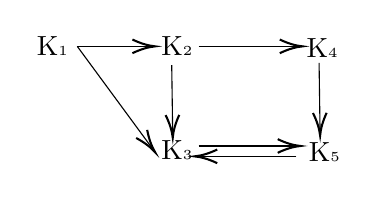
\begin{tikzpicture}[x=0.75pt,y=0.75pt,yscale=-1,xscale=1]
%uncomment if require: \path (0,404); %set diagram left start at 0, and has height of 404
%Straight Lines
\draw    (140,126) -- (175.5,126) ;
\draw [shift={(177.5,126)}, rotate = 180] [color={rgb, 255:red, 0; green, 0; blue, 0 }  ][line width=0.75]    (10.93,-3.29) .. controls (6.95,-1.4) and (3.31,-0.3) .. (0,0) .. controls (3.31,0.3) and (6.95,1.4) .. (10.93,3.29)   ;
%Straight Lines
\draw    (140,126) -- (176.32,175.39) ;
\draw [shift={(177.5,177)}, rotate = 233.67000000000002] [color={rgb, 255:red, 0; green, 0; blue, 0 }  ][line width=0.75]    (10.93,-3.29) .. controls (6.95,-1.4) and (3.31,-0.3) .. (0,0) .. controls (3.31,0.3) and (6.95,1.4) .. (10.93,3.29)   ;
%Straight Lines
\draw    (198.5,126) -- (246.5,126) ;
\draw [shift={(248.5,126)}, rotate = 180] [color={rgb, 255:red, 0; green, 0; blue, 0 }  ][line width=0.75]    (10.93,-3.29) .. controls (6.95,-1.4) and (3.31,-0.3) .. (0,0) .. controls (3.31,0.3) and (6.95,1.4) .. (10.93,3.29)   ;
%Straight Lines
\draw    (256.5,134) -- (256.97,167) ;
\draw [shift={(257,169)}, rotate = 269.18] [color={rgb, 255:red, 0; green, 0; blue, 0 }  ][line width=0.75]    (10.93,-3.29) .. controls (6.95,-1.4) and (3.31,-0.3) .. (0,0) .. controls (3.31,0.3) and (6.95,1.4) .. (10.93,3.29)   ;
%Straight Lines
\draw    (198.5,174) -- (245.5,174) ;
\draw [shift={(247.5,174)}, rotate = 180] [color={rgb, 255:red, 0; green, 0; blue, 0 }  ][line width=0.75]    (10.93,-3.29) .. controls (6.95,-1.4) and (3.31,-0.3) .. (0,0) .. controls (3.31,0.3) and (6.95,1.4) .. (10.93,3.29)   ;
%Straight Lines
\draw    (245.5,179) -- (198.5,179) ;
\draw [shift={(196.5,179)}, rotate = 360] [color={rgb, 255:red, 0; green, 0; blue, 0 }  ][line width=0.75]    (10.93,-3.29) .. controls (6.95,-1.4) and (3.31,-0.3) .. (0,0) .. controls (3.31,0.3) and (6.95,1.4) .. (10.93,3.29)   ;
%Straight Lines
\draw    (185.5,135) -- (185.97,168) ;
\draw [shift={(186,170)}, rotate = 269.18] [color={rgb, 255:red, 0; green, 0; blue, 0 }  ][line width=0.75]    (10.93,-3.29) .. controls (6.95,-1.4) and (3.31,-0.3) .. (0,0) .. controls (3.31,0.3) and (6.95,1.4) .. (10.93,3.29)   ;
% Text Node
\draw (128,126) node  [align=left] {K{\tiny 1}};
% Text Node
\draw (188,126) node  [align=left] {K{\tiny 2}};
% Text Node
\draw (188,176) node  [align=left] {K{\tiny 3}};
% Text Node
\draw (258,127) node  [align=left] {K{\tiny 4}};
% Text Node
\draw (259,177) node  [align=left] {K{\tiny 5}};
\end{tikzpicture}
\end{center}
Message routes can be represented by a matrix $W = w_{ij}$, where $w_{ij} = 0$ except $w_{ij} = 1$ if a message can be sent from $K_{i}$ to $K_{j}$.\[W = \left[\begin{array}{ccccc}
0 & 1 & 1 & 0 & 0 \\ 
0 & 0 & 1 & 1 & 0 \\ 
0 & 0 & 0 & 0 & 1 \\ 
0 & 0 & 0 & 0 & 1 \\ 
0 & 0 & 1 & 0 & 0 \\ 
\end{array}\right]\] In the $r^{th}$ power of this matrix $W^{r} = {w_{ij}(r)}, w_{ij}(r)$ is the number of ways of getting a message from $K_{i}$ to $K_{j}$ in $r$ steps.
\begin{enumerate}
\item Find $W^{2}$. Identify the paths that a message can go from $K_{2}$ to $K_{5}$ in 2 steps
\begin{Schunk}
\begin{Sinput}
> W %*% W
\end{Sinput}
\begin{Soutput}
     [,1] [,2] [,3] [,4] [,5]
[1,]    0    0    1    1    1
[2,]    0    0    0    0    2
[3,]    0    0    1    0    0
[4,]    0    0    1    0    0
[5,]    0    0    0    0    1
\end{Soutput}
\end{Schunk}
The paths are: $K_{2} \rightarrow K_{4} \rightarrow K_{5}$, and $K_{2} \rightarrow K_{3} \rightarrow K_{5}$
\item Find $W^{3}$. Identify the paths that a message can go from $K_{2}$ to $K_{3}$ in 3 steps
\begin{Schunk}
\begin{Sinput}
> W %*% W %*% W
\end{Sinput}
\begin{Soutput}
     [,1] [,2] [,3] [,4] [,5]
[1,]    0    0    1    0    2
[2,]    0    0    2    0    0
[3,]    0    0    0    0    1
[4,]    0    0    0    0    1
[5,]    0    0    1    0    0
\end{Soutput}
\end{Schunk}
The paths are $K_{2} \rightarrow K_{4} \rightarrow K_{5} \rightarrow K_{3}$ and $K_{2} \rightarrow K_{3} \rightarrow K_{5} \rightarrow K_{3}$
\end{enumerate}
\item For $A\underline{x} = \underline{b}$ where $A = \left[\begin{array}{ccc}2 & -2 & -1\\1 & 1 & -2 \\ 1 & 0 & -1\end{array}\right]$ and $\underline{b} = \left[\begin{array}{c}5 \\ 1\\ 4\end{array}\right]$
\begin{enumerate}
\item Find the rank of $A$
\begin{Schunk}
\begin{Sinput}
> as.numeric(Matrix::rankMatrix(A))
\end{Sinput}
\begin{Soutput}
[1] 3
\end{Soutput}
\end{Schunk}
\item Show that $B = \left[\begin{array}{ccc}-1 & -2 & 5 \\ -1 & -1 & 3 \\ -1 & -2 & 4\end{array}\right] = A^{-1}$
\begin{Schunk}
\begin{Sinput}
> solve(A)
\end{Sinput}
\begin{Soutput}
     [,1] [,2] [,3]
[1,]   -1   -2    5
[2,]   -1   -1    3
[3,]   -1   -2    4
\end{Soutput}
\begin{Sinput}
> all.equal(B, solve(A))
\end{Sinput}
\begin{Soutput}
[1] TRUE
\end{Soutput}
\end{Schunk}
\item Solve for $\underline{x}$
\begin{Schunk}
\begin{Sinput}
> solve(A) %*% b
\end{Sinput}
\begin{Soutput}
     [,1]
[1,]   13
[2,]    6
[3,]    9
\end{Soutput}
\end{Schunk}
\end{enumerate}
\end{enumerate}
\end{document}
